\documentclass[leqno]{article}
% Shared mark scheme preamble for resources.danieljsmith.org: the pack
% preamble, unchanged, then the scheme's own layer. A scheme's .tex is
% rendered from its YAML (scripts/README.md, Mark schemes), never edited.
\input{\CurrentFilePath/pack_preamble.tex}

% The page: equal side margins, so the table runs the full width of the
% header rule. The footers' right edge follows the text's.
\geometry{left=0.8in, right=0.8in}
\makeatletter
\renewcommand{\djs@footR}[1]{%
  \put(\dimexpr1in+\hoffset+\oddsidemargin+\textwidth\relax,
    -\dimexpr\paperheight-0.32in\relax){\makebox[0pt][r]{#1}}}
\makeatother

\usepackage[export]{adjustbox}
\usepackage{tabularray}
\definecolor{msGrid}{RGB}{176, 172, 164}
\definecolor{msTint}{RGB}{245, 243, 239}

% The header on every page, the front page included, and the booklet label
% under the contents-page title. \djsQuestionPageStyle stays empty.
\newcommand{\djsSchemeHeader}[1]{%
  \djsPackHeader[markscheme]{\textit{Mark scheme} - #1}%
  \renewcommand{\djsPackTitle}{#1}%
  \renewcommand{\djsBookletLabel}{Mark scheme}%
}

% The front page: the contents heading, spaced as tocloft spaces the packs'
% "Questions", then the contents table. A question's name and page number
% both link to its first page.
\newcommand{\msContentsHeading}{%
  \vskip\cftbeforetoctitleskip
  {\noindent\cfttoctitlefont\contentsname\par}%
  \vskip\cftaftertoctitleskip}
\NewTblrEnviron{mscontents}
\SetTblrInner[mscontents]{
  colspec = {Q[wd=26mm, l] X[l] Q[wd=16mm, c] Q[wd=14mm, r]},
  width = \linewidth,
  rowsep = 4pt, colsep = 6pt,
  hlines = {0.4pt, msGrid}, vlines = {0.4pt, msGrid},
  hline{2} = {2.2pt, scarlet},
  row{1} = {font=\small\bfseries},
  row{Z} = {font=\bfseries},
  column{2} = {font=\small},
}
\newcommand{\msContentsQuestion}[1]{\hyperref[q:#1]{Question #1}}
\newcommand{\msContentsPage}[1]{\hyperref[q:#1]{\pageref*{q:#1}}}
\newcommand{\msSep}{\hspace{0.9em}}

% The conventions pages' layout: headings in the documents' own bold, tables
% ruled and padded as the scheme's, roomy lists.
\newcommand{\msHead}[1]{%
  \par\vspace{18pt}%
  {\noindent\bfseries #1\par}%
  \vspace{6pt}}
\NewTblrEnviron{mstblr}
\SetTblrInner[mstblr]{rowsep = 6pt, colsep = 6pt,
  hlines = {0.4pt, msGrid}, vlines = {0.4pt, msGrid}}
\newenvironment{msList}
  {\begin{itemize}[leftmargin=1.2em, itemsep=5pt, topsep=3pt, parsep=0pt]}
  {\end{itemize}}

% A question's first page: the link target and the PDF bookmark, as
% \questionitem gives the packs.
\newcommand{\msQnum}{}
\newcommand{\msQuestion}[1]{%
  \clearpage
  \renewcommand{\msQnum}{#1}%
  \phantomsection\label{q:#1}%
  \addcontentsline{toc}{subsection}{\protect\djsTocEntry{#1}}}

% The scheme's table: Question 16mm, Scheme the rest, Marks 16mm, Notes
% 44mm; every cell ruled in msGrid; the scarlet rule under the head row. A
% long table has no caption or "continued" foot; a continuation page opens
% with a muted line above the repeated head row. The rules across a part's
% rows, the alternative's tint and the total row are the rendered table's.
\NewTblrTheme{ms}{%
  \DefTblrTemplate{firsthead}{default}{}%
  \DefTblrTemplate{middlehead,lasthead}{default}{%
    {\small\itshape\color{djsMuted}Question \msQnum\ continued\par}%
    \vspace{6pt}}%
  \DefTblrTemplate{firstfoot,middlefoot,lastfoot}{default}{}%
}
\NewTblrEnviron{msscheme}
\SetTblrOuter[msscheme]{long, theme=ms, entry=none, label=none}
\SetTblrInner[msscheme]{
  colspec = {Q[wd=16mm, l] X[l] Q[wd=16mm, c] Q[wd=44mm, l]},
  width = \linewidth,
  rowsep = 6pt, colsep = 6pt,
  rowhead = 1,
  vlines = {0.4pt, msGrid},
  hline{1} = {0.4pt, msGrid}, hline{2} = {2.2pt, scarlet},
  hline{Z} = {0.4pt, msGrid},
  column{1} = {font=\bfseries}, column{3} = {font=\bfseries},
  column{4} = {font=\small},
  row{1} = {rowsep=4pt, font=\small\bfseries},
}

% Two marks on a row: each note starts with its code.
\newcommand{\msNote}[2]{\textbf{#1}\enspace #2}
% A full-row figure: the worked solution's own picture, scaled uniformly and
% only down, to the table less the Question column. The picture is drawn
% with the line width it has in the solutions document, at its list depth
% there (the optional argument, 1 by default: a part's working), so one
% sized by \linewidth keeps its size; tabularray sets the cell's \linewidth
% to the cell's measured width, which would shrink it at every pass. The
% widths are measured once, in a solution box at the packs' text width
% (pack_preamble.tex's margins, 0.8in and 1in).
\newlength{\msSpanW}
\makeatletter
\newcommand{\ms@keepLW}[1]{%
  \expandafter\xdef\csname ms@solnLW@#1\endcsname{\the\linewidth}}
\AtBeginDocument{%
  \setlength{\msSpanW}{\dimexpr\textwidth-16mm-28pt\relax}%
  \setbox\z@\vbox{%
    \begin{minipage}{\dimexpr\paperwidth-1.8in\relax}
      \begin{djsSolution}
        \ms@keepLW{0}%
        \begin{enumerate}\item \ms@keepLW{1}%
        \begin{enumerate}\item \ms@keepLW{2}%
        \begin{enumerate}\item \ms@keepLW{3}%
        \end{enumerate}\end{enumerate}\end{enumerate}
      \end{djsSolution}
    \end{minipage}}}
\newcommand{\msFigure}[2][1]{%
  \adjustbox{max width=\msSpanW, max totalheight=0.6\textheight, valign=t}{%
    \hsize=\csname ms@solnLW@#1\endcsname
    \linewidth=\hsize
    #2}}
\makeatother
% A figure mark's feature, in the Scheme column.
\newcommand{\msFeature}[1]{\textit{#1}}
% An alternative's title row.
\newcommand{\msAlternative}[1]{\textit{Alternative:} #1}
% Drafts only: a queried mark's code, the query's why under its note, and a
% flag in its part's place.
\newcommand{\msQueried}[2]{#1~\(\to\) #2?}
\newcommand{\msQuery}[1]{{\itshape\color{djsMuted}Query: #1}}
\newcommand{\msFlag}[2]{\textbf{#1:}\enspace #2}


\djsSchemeHeader{Loci and Regions in the Argand Diagram}
\djsSitePath{Core Pure}{Complex Numbers}

\djsLastUpdated{24 October 2026}
\begin{document}
\djsSetQuestionCount{10}
\djsAddMarks{1}{6}
\djsAddMarks{2}{6}
\djsAddMarks{3}{10}
\djsAddMarks{4}{11}
\djsAddMarks{5}{11}
\djsAddMarks{6}{12}
\djsAddMarks{7}{7}
\djsAddMarks{8}{8}
\djsAddMarks{9}{9}
\djsAddMarks{10}{7}
\vspace*{6pt}
\djsContentsTitle
\vspace{30pt}
\msContentsHeading
\begin{mscontents}{}
Question & Marks by part & Marks & Page \\
\msContentsQuestion{1} & (a)\,2\msSep (b)\,2\msSep (c)\,2 & 6 & \msContentsPage{1} \\
\msContentsQuestion{2} & (a)\,2\msSep (b)\,1\msSep (c)\,3 & 6 & \msContentsPage{2} \\
\msContentsQuestion{3} & (a)(i)\,1\msSep (a)(ii)\,1\msSep (b)\,1\msSep (c)\,3\msSep (d)\,4 & 10 & \msContentsPage{3} \\
\msContentsQuestion{4} & (a)(i)\,2\msSep (a)(ii)\,3\msSep (b)(i)\,3\msSep (b)(ii)\,3 & 11 & \msContentsPage{4} \\
\msContentsQuestion{5} & (a)\,2\msSep (b)(i)\,2\msSep (b)(ii)\,2\msSep (c)\,5 & 11 & \msContentsPage{5} \\
\msContentsQuestion{6} & (a)\,5\msSep (b)\,5\msSep (c)\,2 & 12 & \msContentsPage{6} \\
\msContentsQuestion{7} & & 7 & \msContentsPage{7} \\
\msContentsQuestion{8} & (a)\,2\msSep (b)(i)\,2\msSep (b)(ii)\,4 & 8 & \msContentsPage{8} \\
\msContentsQuestion{9} & (a)\,2\msSep (b)\,7 & 9 & \msContentsPage{9} \\
\msContentsQuestion{10} & (a)\,2\msSep (b)\,1\msSep (c)\,2\msSep (d)\,2 & 7 & \msContentsPage{10} \\
\SetCell[c=2]{r} Total & & 87 & \\
\end{mscontents}
\newpage
% The conventions pages, shared by every pack's mark scheme: one source of
% truth, \input after the front page, with no strand or pack logic. The keys
% on the first side, the rules on the second. The scheme layer defines
% \msHead, msList and mstblr.
\vspace*{6pt}%
{\noindent\cfttoctitlefont Reading the mark scheme\par}%
\vspace{10pt}%
These rules apply throughout, unless a note says otherwise.

\msHead{Marks}
Every mark is worth one, so \textbf{M1 A1} on a row is two marks. Only marks
coded ft follow through.\par
\vspace{10pt}%
\begin{mstblr}{
  colspec = {Q[wd=15mm, l] X[l]},
  width = \linewidth,
  hline{2} = {2.2pt, scarlet},
  column{1} = {font=\bfseries},
  row{1} = {font=\small\bfseries, rowsep=4pt},
}
Code & Meaning \\
M1 & Method: a correct method, applied to this question. A slip doesn't cost it if the method is clear. A formula must be used, not just quoted. \\
dM1 & Dependent method: as M1, but only if the method mark before it was earned, unless its note names another. \\
A1 & Accuracy: a correct answer or step. It needs the method mark it follows. \\
A1ft & As A1, following through from an earlier answer that the note names. \\
A1~AG & The last mark of a part whose answer is printed in the question: complete working, with no errors. \\
B1 & A correct value, fact or statement. It needs no method mark. \\
B1ft & As B1, following through from an earlier answer that the note names. \\
E1 & A written explanation, interpretation or conclusion. Concluding a proof by induction needs every earlier mark. \\
\end{mstblr}

\msHead{Abbreviations}
ft and AG qualify a code in the Marks column. The others appear in the
notes.\par
\vspace{10pt}%
\begin{mstblr}{
  colspec = {Q[wd=17mm, l] X[l] Q[wd=15mm, l] X[l]},
  width = \linewidth,
  column{1} = {font=\bfseries}, column{3} = {font=\bfseries},
}
ft & follow through & AG & answer given in the question \\
cao & correct answer only, with no follow-through & cso & correct solution only: no errors in the part \\
oe & or an equivalent form & awrt & any answer that rounds to this value \\
soi & seen, or implied by later working & isw & ignore working after a correct answer \\
SC & special case: credit outside the main method & their & the student's own earlier value \\
condone & a slip that doesn't cost the mark & [\;\,] & working the mark doesn't need \\
s.f. & significant figures & d.p. & decimal places \\
\end{mstblr}

\newpage
\msHead{Reading the scheme}
\begin{msList}
\item Each row is a line of working, with the marks it earns beside it.
  Where a row carries two marks, each note starts with its code.
\item \textbf{[\textit{n}]} ends each part with its total.
\item A shaded \textit{Alternative} is a second method for the same total.
  Mark an answer by the method it follows.
\item Any other valid method earns the equivalent marks, unless the question
  names a method or says \textit{hence}.
\item A sketch earns one B1 for each feature named below its figure.
\end{msList}

\msHead{Accuracy and answers}
\begin{msList}
\item Unless a question says otherwise, give answers to 3 significant
  figures, and angles in degrees to 1 decimal place. Angles in radians take
  3 significant figures.
\item A final answer with more figures is accepted if it rounds to the
  scheme's value; one with fewer is not. An answer spoiled by rounding too
  early loses its accuracy mark.
\item Where a question asks for an exact answer, a decimal loses the final
  accuracy mark. Otherwise either is accepted.
\item Wrong or missing units cost nothing unless the question asks for them.
\item A correct answer with no working earns full marks, unless the question
  needs the working: show that, prove, hence, a method it names, or an exact
  answer. A wrong answer with no working earns nothing. Calculator answers
  are treated the same way.
\item A correct answer, once reached, isn't spoiled by later working (isw).
\end{msList}

\msHead{Value of $\boldsymbol{g}$}
\begin{msList}
\item Take $g = 9.8\,\mathrm{m\,s^{-2}}$ unless a question states a value,
  which is then the only one accepted. Answers that use $g = 9.8$ may be
  given to 2 or 3 significant figures.
\item Where a question doesn't state $g$, an answer worked with $g = 10$
  throughout earns the same marks, keeping any value printed in the
  question. The worked solutions list the final answers with $g = 10$.
\end{msList}


\msQuestion{1}
\begin{msscheme}{
  hline{3,5-7,9-10} = {2-Z}{0.4pt, msGrid},
  hline{4,8,11} = {0.4pt, msGrid},
  row{11} = {font=\bfseries},
}
Question & Scheme & Marks & Notes \\
1(a) & {\(\{z \in \mathbb{C} : |z + 2 - i| = 4\}\)} & B1 B1 & {\msNote{B1}{\(|z + 2 - i|\) oe, such as \(|z - (-2 + i)|\).}\\ \msNote{B1}{Equal to 4, inside set braces with \(z\) defined by a colon or bar. Condone \(\in \mathbb{C}\) omitted.}} \\
\nopagebreak & & [2] & \\
1(b) & \SetCell[c=3]{c} \msFigure{\begin{tikzpicture}[scale=0.75]
\def\xmin{-6.3}
\def\xmax{4.7}
\def\ymin{-4.3}
\def\ymax{6.3}
\def\cx{-2}
\def\cy{1}
\def\rad{4}
\coordinate (O) at (0,0);
\coordinate (C) at (-2,1);
\coordinate (A) at (2,1);
\coordinate (B) at (-1,3);
\draw[-{Stealth[length=3mm]}, thick] (\xmin,0) -- (\xmax,0) node[right] {$\mathrm{Re}(z)$};
\draw[-{Stealth[length=3mm]}, thick] (0,\ymin) -- (0,\ymax) node[above] {$\mathrm{Im}(z)$};
\draw[thick] (C) circle (\rad);
\draw[thick] (-3.5,-4) -- (3.3,6.2) node[above right] {$L$};
\draw[dashed] (A) -- (B);
\fill (C) circle (2pt);
\fill (A) circle (2pt);
\fill (B) circle (2pt);
\draw[thick] (\cx,0.12) -- (\cx,-0.12);
\draw[thick] (0.12,\cy) -- (-0.12,\cy);
\node[below left] at (O) {$O$};
\node[below] at (\cx,0) {$-2$};
\node[right] at (0.12,\cy) {$1$};
\node[above left] at (C) {$-2+i$};
\node[below right] at (A) {$2+i$};
\node[above left] at (B) {$-1+3i$};
\end{tikzpicture}} & & \\
& \msFeature{Shape} & B1 & {Straight line, drawn as the perpendicular bisector of the segment from \(2 + i\) to \(-1 + 3i\).} \\
& \msFeature{Labelled point} & B1 & {Through \(\left(\frac12, 2\right)\) with positive gradient, about \(\frac32\), crossing the Re axis between \(-2\) and \(O\); labelled \(L\).} \\
\nopagebreak & & [2] & \\
1(c) & {\(z = x + 5i \Rightarrow z + 1 - 2i = (x + 1) + 3i\)\\[4pt] \(\tan\frac{2\pi}{3} = \frac{3}{x + 1} \Rightarrow x = \ldots\)} & M1 & {Uses \(\mathrm{Im}(z) = 5\) and \(\tan\frac{2\pi}{3}\) or \(\tan\frac{\pi}{3}\) as the ratio of imaginary to real parts of \(z + 1 - 2i\), solving for \(x\). Condone sign slips.} \\
& {\(z = -1 - \sqrt{3} + 5i\)} & A1 & {oe, or awrt \(-2.73 + 5i\), as a complex number.} \\
\nopagebreak & & [2] & \\
\nopagebreak \SetCell[c=2]{r} Total for Question 1 & & 6 & \\
\end{msscheme}

\msQuestion{2}
\begin{msscheme}{
  hline{3-5,7-8,10-12} = {2-Z}{0.4pt, msGrid},
  hline{6,9,13} = {0.4pt, msGrid},
  row{13} = {font=\bfseries},
}
Question & Scheme & Marks & Notes \\
2(a) & \SetCell[c=3]{c} \msFigure{\begin{tikzpicture}[scale=0.7]
\def\cx{2}
\def\cy{4}
\def\rad{3}
\draw[-{Stealth[length=3mm]}, thick] (-2.2,0) -- (7.7,0) node[right] {$\mathrm{Re}(z)$};
\draw[-{Stealth[length=3mm]}, thick] (0,-1.2) -- (0,7.7) node[above] {$\mathrm{Im}(z)$};
\foreach \x in {-2,-1,1,2,3,4,5,6,7} {
  \draw (\x,0.12) -- (\x,-0.12);
  \node[below] at (\x,-0.12) {$\x$};
}
\foreach \y in {-1,1,2,3,4,5,6,7} {
  \draw (0.12,\y) -- (-0.12,\y);
  \node[left] at (-0.12,\y) {$\y$};
}
\node[below left] at (0,0) {$O$};
\draw[thick] (\cx,\cy) circle (\rad);
\fill (\cx,\cy) circle (1.5pt);
\node[above left] at (\cx,\cy) {$2+4i$};
\end{tikzpicture}} & & \\
& \msFeature{Shape} & B1 & {A closed circle, freehand accepted.} \\
& \msFeature{Centre and radius} & B1 & {Centre at \(2 + 4i\) and radius 3, shown by position against the scales or by labels.} \\
\nopagebreak & & [2] & \\
2(b) & \SetCell[c=3]{c} \msFigure{\begin{tikzpicture}[scale=0.7]
\def\cx{2}
\def\cy{4}
\def\rad{3}
\draw[-{Stealth[length=3mm]}, thick] (-2.2,0) -- (7.7,0) node[right] {$\mathrm{Re}(z)$};
\draw[-{Stealth[length=3mm]}, thick] (0,-1.2) -- (0,7.7) node[above] {$\mathrm{Im}(z)$};
\foreach \x in {-2,-1,1,2,3,4,5,6,7} {
  \draw (\x,0.12) -- (\x,-0.12);
  \node[below] at (\x,-0.12) {$\x$};
}
\foreach \y in {-1,1,2,3,4,5,6,7} {
  \draw (0.12,\y) -- (-0.12,\y);
  \node[left] at (-0.12,\y) {$\y$};
}
\node[below left] at (0,0) {$O$};
\draw[thick] (\cx,\cy) circle (\rad);
\fill (\cx,\cy) circle (1.5pt);
\node[above left] at (\cx,\cy) {$2+4i$};
\draw[thick] (1,0) -- (7,6);
\draw[fill=white] (1,0) circle (1.7pt);
\end{tikzpicture}} & & \\
& \msFeature{Half-line} & B1 & {Half-line from \(1\) on the real axis at \(\frac{\pi}{4}\), through about \((5, 4)\), going up and right only; start shown excluded or not marked included.} \\
\nopagebreak & & [1] & \\
2(c) & {\((x-2)^2 + (y-4)^2 = 9\), \(y = x - 1\)\\[4pt] \(\Rightarrow (x-2)^2 + (x-5)^2 = 9 \Rightarrow x = \ldots\)} & M1 & {Substitutes the line into a circle equation of the form \((x-2)^2 + (y-4)^2 = 9\), or eliminates \(x\), and solves the quadratic by any means. Condone slips.} \\
& {\(x = 5 \Rightarrow 5 + 4i\)} & A1 & {\(5 + 4i\) or \((5, 4)\) taken as the furthest point; \((2, 1)\) need not be found.} \\
& {\(|w|_{\max} = \sqrt{5^2 + 4^2} = \sqrt{41}\)} & A1 & {\(\sqrt{41}\) or awrt 6.40.} \\
\nopagebreak & & [3] & \\
\nopagebreak \SetCell[c=2]{r} Total for Question 2 & & 6 & \\
\end{msscheme}

\msQuestion{3}
\begin{msscheme}{
  hline{3,5,7-8,10-12,14-17} = {2-Z}{0.4pt, msGrid},
  hline{4,6,9,13,18} = {0.4pt, msGrid},
  row{18} = {font=\bfseries},
}
Question & Scheme & Marks & Notes \\
3(a)(i) & {\((4, -3)\)} & B1 & {Accept \(4 - 3i\).} \\
\nopagebreak & & [1] & \\
3(a)(ii) & {\(8\)} & B1 & \\
\nopagebreak & & [1] & \\
3(b) & \SetCell[c=3]{c} \msFigure{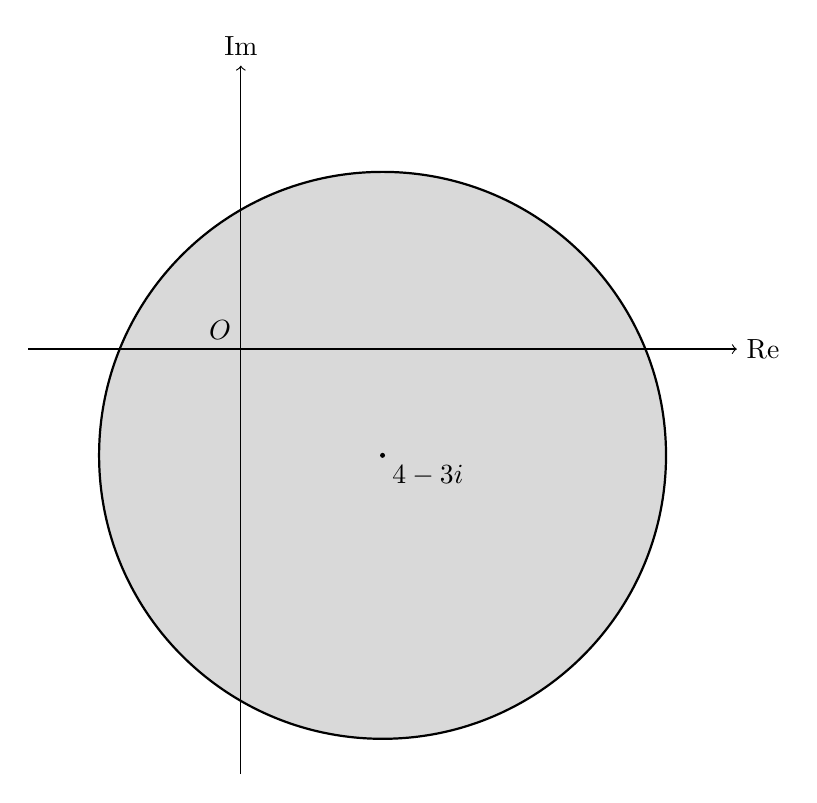
\begin{tikzpicture}[scale=0.45]
  \def\cx{4}
  \def\cy{-3}
  \def\rad{8}
  \fill[gray!30] (\cx,\cy) circle (\rad);
  \draw[->] (-6,0) -- (14,0) node[right] {Re};
  \draw[->] (0,-12) -- (0,8) node[above] {Im};
  \node[above left] at (0,0) {$O$};
  \draw[thick] (\cx,\cy) circle (\rad);
  \fill (\cx,\cy) circle (2pt);
  \node[below right] at (\cx,\cy) {$4-3i$};
\end{tikzpicture}} & & \\
& \msFeature{Shading} & B1 & {Interior of a circle shaded, centre \(4 - 3i\) in the fourth quadrant, enclosing \(O\), with the centre or radius 8 indicated.} \\
\nopagebreak & & [1] & \\
3(c) & {\(|4 - 3i| = \sqrt{4^2 + 3^2} = 5\)} & B1 & \\
& {\(|z|_{\max} = \their{5} + 8 = \ldots\)} & M1 & {Adds the radius to their distance from \(O\) to the centre, or maximises \(|z|\) on the circle by another valid method.} \\
& {\(13\)} & A1 & \\
\nopagebreak & & [3] & \\
3(d) & {\(x + y = 9\), \((x - 4)^2 + (y + 3)^2 = 64\)\\[4pt] \(\Rightarrow x^2 - 16x + 48 = 0 \Rightarrow x = \ldots\)} & M1 & {Combines a line through \((3, 6)\) of gradient \(\pm 1\) with their circle equation and solves for the intersections by any means. Condone sign slips.} \\
& {\((4, 5)\), \((12, -3)\)\\[4pt] \(\Rightarrow \angle PCQ = \frac{\pi}{2}\)} & A1 & {Angle at the centre \(\frac{\pi}{2}\) or \(90^\circ\), from correct intersection points.} \\
& {\(\text{Area} = \tfrac12 \times 8^2 \times \their{\tfrac{\pi}{2}}\)\\[4pt] \(\phantom{\text{Area}} - \tfrac12 \times 8^2 \times \sin\their{\tfrac{\pi}{2}}\)} & dM1 & {Uses sector minus triangle, \(\frac12 r^2(\theta - \sin\theta)\), with \(r = 8\) and their angle at the centre.} \\
& {\(= 16\pi - 32 = 18.3\)} & A1 & {awrt 18.3.} \\
\nopagebreak & & [4] & \\
\nopagebreak \SetCell[c=2]{r} Total for Question 3 & & 10 & \\
\end{msscheme}

\msQuestion{4}
\begin{msscheme}{
  hline{3,5-6,8-11,13-15} = {2-Z}{0.4pt, msGrid},
  hline{4,7,12,16} = {0.4pt, msGrid},
  row{16} = {font=\bfseries},
}
Question & Scheme & Marks & Notes \\
4(a)(i) & {\(|z - (-2 + 4i)| = 3\)\\[4pt] \(|z + 2 - 4i| = 3\)} & B1 B1 & {\msNote{B1}{\(|z - (-2 + 4i)|\) or \(|z + 2 - 4i|\) seen, with any right-hand side.}\\ \msNote{B1}{Correct equation in any modulus form.}} \\
\nopagebreak & & [2] & \\
4(a)(ii) & {\(|z + 2 - 4i| < 3\)} & B1 & {With any inequality or equals sign.} \\
& {\(|z - (2 + 6i)| < 4\)} & B1 B1 & {\msNote{B1}{With any inequality or equals sign.}\\ \msNote{B1}{Strict \(<\) in both, on inequalities for both circles.}} \\
\nopagebreak & & [3] & \\
4(b)(i) & \SetCell[c=3]{c} \msFigure[2]{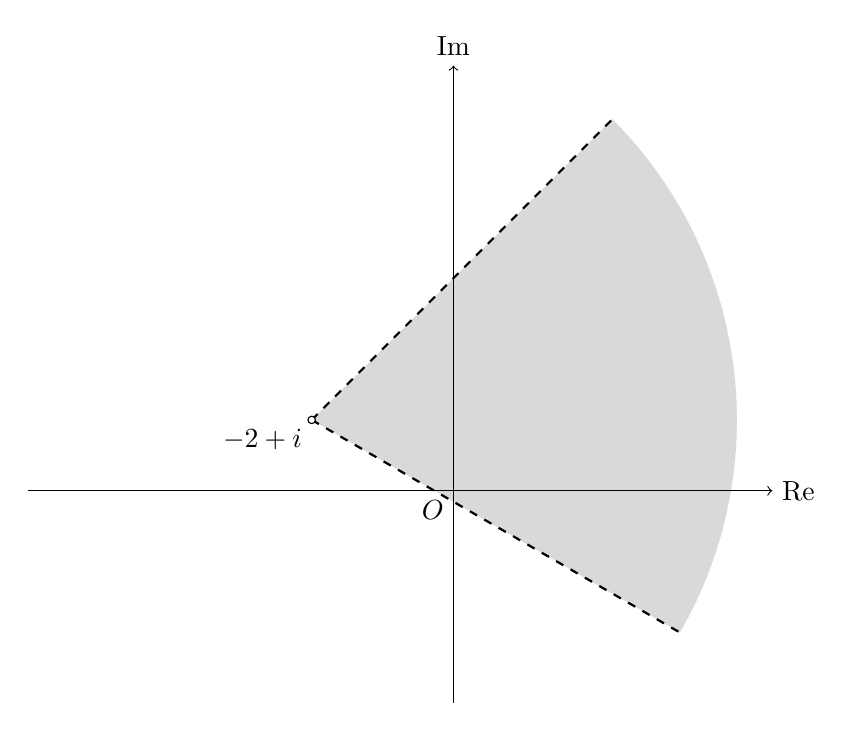
\begin{tikzpicture}[scale=0.9]
  \def\cx{-2}
  \def\cy{1}
  \def\R{6}
  \fill[gray!30] (\cx,\cy) -- ++(-30:\R) arc (-30:45:\R) -- cycle;
  \draw[->] (-6,0) -- (4.5,0) node[right] {Re};
  \draw[->] (0,-3) -- (0,6) node[above] {Im};
  \node[below left] at (0,0) {$O$};
  \draw[thick,dashed] (\cx,\cy) -- ++(-30:\R);
  \draw[thick,dashed] (\cx,\cy) -- ++(45:\R);
  \draw[fill=white] (\cx,\cy) circle (1.5pt);
  \node[below left] at (\cx,\cy) {$-2+i$};
\end{tikzpicture}} & & \\
& \msFeature{Half-line} & B1 & {Half-line from \(-2 + i\) at \(\frac{\pi}{4}\) above the positive real direction; angle labelled or clearly in proportion.} \\
& \msFeature{Half-line} & B1 & {Half-line from \(-2 + i\) at \(\frac{\pi}{6}\) below the positive real direction; angle labelled or clearly in proportion.} \\
& \msFeature{Shading} & B1 & {Region between the half-lines, to the right of \(-2 + i\), shaded or labelled. Condone solid boundaries and an unmarked vertex.} \\
\nopagebreak & & [3] & \\
4(b)(ii) & {\(z + 2 - i = 3 + 4i \Rightarrow \arg(3 + 4i) = \ldots\)} & M1 & {Substitutes \(1 + 5i\) into \(z + 2 - i\) and attempts its argument, or the gradient from \(-2 + i\) to \(1 + 5i\).} \\
& {\(\arctan\frac43 \approx 0.927\)} & A1 & {\(\arctan\frac43\), awrt 0.927 or 53.1°, or gradient \(\frac43\).} \\
& {\(0.927 > \frac{\pi}{4} \approx 0.785\)\\[4pt] \(1 + 5i\) is not in the region} & A1ft & {ft their argument or gradient. Compares with \(\frac{\pi}{4}\) (or \(\tan\frac{\pi}{4} = 1\)), and with \(-\frac{\pi}{6}\) where needed, and concludes correctly.} \\
\nopagebreak & & [3] & \\
\nopagebreak \SetCell[c=2]{r} Total for Question 4 & & 11 & \\
\end{msscheme}

\msQuestion{5}
\begin{msscheme}{
  hline{3-4,6-8,10-11,13-17} = {2-Z}{0.4pt, msGrid},
  hline{5,9,12,18} = {0.4pt, msGrid},
  row{18} = {font=\bfseries},
}
Question & Scheme & Marks & Notes \\
5(a) & {\(|2+2\sqrt{3}i| = \sqrt{2^2 + (2\sqrt{3})^2}\)} & M1 & {Squares the real and imaginary parts, adds and takes the square root. Condone one slip in squaring.} \\
& {\(= 4\)} & A1 & \\
\nopagebreak & & [2] & \\
5(b)(i) & \SetCell[c=3]{c} \msFigure[2]{\begin{tikzpicture}[scale=0.8]
\coordinate (O) at (0,0);
\coordinate (C) at (2,-3.464101615);
\coordinate (W) at (3,-1.732050808);
\draw[thick, -{Stealth[length=3mm]}] (-2.8,0) -- (6.8,0) node[right] {$\mathrm{Re}(z)$};
\draw[thick, -{Stealth[length=3mm]}] (0,-5.8) -- (0,3.8) node[above] {$\mathrm{Im}(z)$};
\draw[thick] (C) circle (2);
\fill (C) circle (2pt);
\draw[thick] (2,0.12) -- (2,-0.12);
\draw[thick] (0.12,-3.464101615) -- (-0.12,-3.464101615);
\node[below left] at (O) {$O$};
\node[below] at (2,0) {$2$};
\node[left] at (0,-3.464101615) {$-2\sqrt{3}$};
\node[right] at (C) {$2-2\sqrt{3}i$};
\node[above right] at (4,-2.5) {$L$};
\end{tikzpicture}} & & \\
& \msFeature{Shape} & B1 & {A circle drawn wholly below the real axis.} \\
& \msFeature{Centre and radius} & B1 & {Centre \(2-2\sqrt{3}i\) or \((2, -2\sqrt{3})\) indicated, and the circle touching the imaginary axis at \(-2\sqrt{3}i\).} \\
\nopagebreak & & [2] & \\
5(b)(ii) & {\(\sin\alpha = \frac{2}{4} \Rightarrow \alpha = \frac{\pi}{6}\)\\[4pt] \(\arg w = -\frac{\pi}{3} + \alpha\)} & M1 & {Uses the tangent from \(O\) to \(L\), adding the angle between \(OC\) and the tangent to their \(\arg\) of the centre, or finds the tangent's gradient by any method.} \\
& {\(\arg w = -\frac{\pi}{6}\)} & A1 & {In terms of \(\pi\).} \\
\nopagebreak & & [2] & \\
5(c) & {\(|2+2\sqrt{3}i| = 4\), \(\arg = \arctan\sqrt{3} = \ldots\)} & M1 & {Finds the modulus and attempts an argument by trigonometry on the real and imaginary parts. The modulus may come from (a).} \\
& {\(z^4 = 4e^{i\pi/3}\)} & A1 & {oe, such as \(4\left(\cos\frac{\pi}{3} + i\sin\frac{\pi}{3}\right)\).} \\
& {\(r = \their{4}^{1/4}\), \(\theta = \dfrac{\their{\frac{\pi}{3}} + 2k\pi}{4}\)} & M1 & {Takes the fourth root of their modulus, and divides their argument plus \(2k\pi\) by 4 for at least two values of \(k\), or adds multiples of \(\frac{\pi}{2}\) to one root's argument.} \\
& {\(z = \sqrt{2}\,e^{i\pi/12},\ \sqrt{2}\,e^{7\pi i/12}\)} & A1 & {Any two correct roots; arguments need not be in range. Modulus \(\sqrt{2}\) oe or awrt 1.41, arguments exact or awrt.} \\
& {\(z = \sqrt{2}\,e^{-11\pi i/12},\ \sqrt{2}\,e^{-5\pi i/12}\)} & A1 & {All four roots in the form \(re^{i\theta}\) with \(-\pi < \theta \leq \pi\), and no others.} \\
\nopagebreak & & [5] & \\
\nopagebreak \SetCell[c=2]{r} Total for Question 5 & & 11 & \\
\end{msscheme}

\msQuestion{6}
\begin{msscheme}{
  hline{3-6,8-13,15-17} = {2-Z}{0.4pt, msGrid},
  hline{7,14,18} = {0.4pt, msGrid},
  row{18} = {font=\bfseries},
}
Question & Scheme & Marks & Notes \\
6(a) & {\((x-1)^2+(y-1)^2\)\\[4pt] \(\phantom{(x-1)^2} = \frac14\left((x-4)^2+(y-1)^2\right)\)} & M1 A1 & {\msNote{M1}{Writes both moduli in terms of \(x\) and \(y\) and squares both sides. Condone sign slips and the \(\frac12\) left unsquared.}\\ \msNote{A1}{Any correct equation without square roots.}} \\
& {\(3x^2+3y^2-6y-9=0\)\\[4pt] \(\Rightarrow x^2+(y-1)^2 = \ldots\)} & dM1 & {Expands and collects to \(x^2+y^2+ax+by+c=0\) or a multiple, then completes the square or uses centre \(\left(-\frac a2,-\frac b2\right)\). Condone arithmetic slips.} \\
& {\(x^2+(y-1)^2=4\), a circle} & A1 & {Or \(x^2+y^2-2y-3=0\), with the locus stated to be a circle.} \\
& {Centre \((0,1)\), radius \(2\)} & A1 & {Both, cso.} \\
\nopagebreak & & [5] & \\
6(b) & \SetCell[c=3]{c} \msFigure{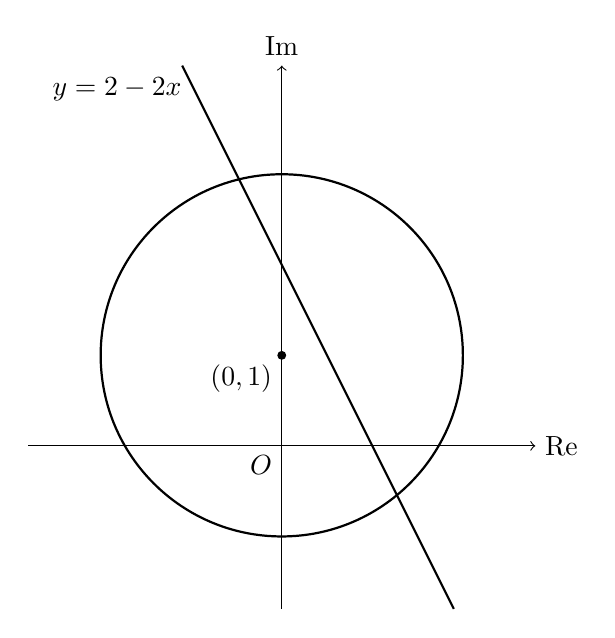
\begin{tikzpicture}[scale=1.15]
\def\cx{0}
\def\cy{1}
\def\rad{2}
\draw[->] (-2.8,0) -- (2.8,0) node[right] {Re};
\draw[->] (0,-1.8) -- (0,4.2) node[above] {Im};
\node[below left] at (0,0) {$O$};
\draw[thick] (\cx,\cy) circle (\rad);
\draw[thick] (-1.1,4.2) -- (1.9,-1.8);
\fill (\cx,\cy) circle (1.4pt);
\node[below left] at (\cx,\cy) {$(0,1)$};
\node[above left] at (-1.0,3.7) {$y=2-2x$};
\end{tikzpicture}} & & \\
& \msFeature{Shape} & B1 & {A circle, crossing both axes twice.} \\
& \msFeature{Centre and radius} & B1 & {Centre \((0,1)\) marked, and radius 2 shown or the circle through \(3i\) and \(-i\).} \\
& {\((x-2)^2+(y-3)^2=(x+2)^2+(y-1)^2\)\\[4pt] \(\Rightarrow -8x-4y+8=0\)} & M1 & {Squares the moduli in terms of \(x\) and \(y\) and simplifies to a linear equation, or finds the perpendicular bisector of \((2,3)\) and \((-2,1)\). Condone sign slips.} \\
& {\(y=2-2x\)} & A1 & {oe, such as \(2x+y=2\).} \\
& {Line \(y=2-2x\) on the same diagram} & B1 & {Straight line of negative gradient through \((1,0)\) and \((0,2)\), cutting the circle twice. Intercepts need not be labelled.} \\
\nopagebreak & & [5] & \\
6(c) & \SetCell[c=3]{c} \msFigure{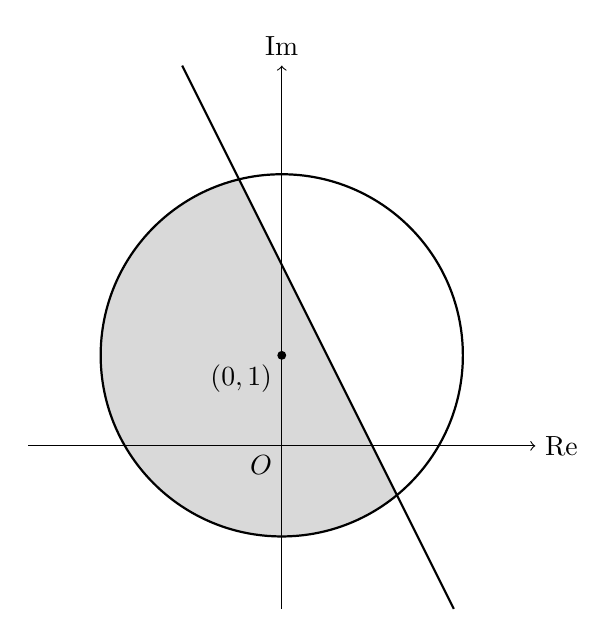
\begin{tikzpicture}[scale=1.15]
\def\cx{0}
\def\cy{1}
\def\rad{2}
\begin{scope}
  \clip (\cx,\cy) circle (\rad);
  \fill[gray!30] (-3,-2) -- (2,-2) -- (-1,4) -- (-3,4) -- cycle;
\end{scope}
\draw[->] (-2.8,0) -- (2.8,0) node[right] {Re};
\draw[->] (0,-1.8) -- (0,4.2) node[above] {Im};
\node[below left] at (0,0) {$O$};
\draw[thick] (\cx,\cy) circle (\rad);
\draw[thick] (-1.1,4.2) -- (1.9,-1.8);
\fill (\cx,\cy) circle (1.4pt);
\node[below left] at (\cx,\cy) {$(0,1)$};
\end{tikzpicture}} & & \\
& \msFeature{Shading} & B1 & {Shaded region lies inside the circle.} \\
& \msFeature{Shading} & B1 & {Shading on the side of the line containing \(O\), with only the intersection of the two regions shaded.} \\
\nopagebreak & & [2] & \\
\nopagebreak \SetCell[c=2]{r} Total for Question 6 & & 12 & \\
\end{msscheme}

\msQuestion{7}
\begin{msscheme}{
  hline{3-8} = {2-Z}{0.4pt, msGrid},
  hline{9} = {0.4pt, msGrid},
  row{9} = {font=\bfseries},
}
Question & Scheme & Marks & Notes \\
7 & {\((x-2)^2 + (y+1)^2 = 9\)} & B1 & {oe, such as \(x^2 + y^2 - 4x + 2y - 4 = 0\).} \\
& {\((x+1)^2 + (y-11)^2 = 9\left((x+1)^2 + (y-3)^2\right)\)} & M1 & {Writes both moduli in terms of \(x\) and \(y\) and squares both sides. Condone sign slips.} \\
& {\((x+1)^2 + (y-2)^2 = 9\)} & A1 & {oe, such as \(x^2 + y^2 + 2x - 4y - 4 = 0\).} \\
& {\((x-2)^2 + (y+1)^2 = (x+1)^2 + (y-2)^2\)\\[4pt] \(\Rightarrow -6x + 6y = 0\)} & M1 & {Subtracts their circle equations, each with equal coefficients of \(x^2\) and \(y^2\), to reach a linear equation in \(x\) and \(y\). Condone sign slips.} \\
& {\(y = x\)} & A1 & \\
& {\((x-2)^2 + (x+1)^2 = 9\)\\[4pt] \(\Rightarrow x^2 - x - 2 = 0 \Rightarrow x = \ldots\)} & dM1 & {Substitutes their linear equation into either circle and solves the three-term quadratic by any means, leading to \(x = \ldots\) or \(y = \ldots\).} \\
& {\((2, 2)\) and \((-1, -1)\)} & A1 & {Both points and no others.} \\
\nopagebreak \SetCell[c=2]{r} Total for Question 7 & & 7 & \\
\end{msscheme}

\msQuestion{8}
\begin{msscheme}{
  hline{3-5,7-8,10-13} = {2-Z}{0.4pt, msGrid},
  hline{6,9,14} = {0.4pt, msGrid},
  row{14} = {font=\bfseries},
}
Question & Scheme & Marks & Notes \\
8(a) & \SetCell[c=3]{c} \msFigure{\begin{tikzpicture}[scale=1]
    \def\cx{3}
    \def\cy{1}
    \def\rad{1}
\draw[->, thick] (-2.2,0) -- (6.7,0) node[right] {$\mathrm{Re}(z)$};
\draw[->, thick] (0,-2.2) -- (0,5.7) node[above] {$\mathrm{Im}(z)$};
\foreach \x in {-2,-1,1,2,3,4,5,6} {
  \draw (\x,0.12) -- (\x,-0.12) node[below] {$\x$};
}
\foreach \y in {-2,-1,1,2,3,4,5} {
  \draw (0.12,\y) -- (-0.12,\y) node[left] {$\y$};
}
    \draw[thick] (\cx,\cy) circle (\rad);
    \fill (\cx,\cy) circle (1.5pt);
    \node[above right] at (\cx,\cy) {$3+i$};
\node[below left] at (0,0) {$O$};
\end{tikzpicture}} & & \\
& \msFeature{Shape} & B1 & {A circle, roughly round.} \\
& \msFeature{Centre and radius} & B1 & {Centre at \(3 + i\) and radius 1, shown by position against the scales or by labels.} \\
\nopagebreak & & [2] & \\
8(b)(i) & {\((x-3)^2 + (mx-1)^2 = 1\)\\[4pt] \(\Rightarrow (1+m^2)x^2 - (6+2m)x + 9 = 0\)\\[4pt] \((6+2m)^2 - 36(1+m^2) = 0 \Rightarrow m = \ldots\)} & M1 & {Uses a tangency condition, such as a zero discriminant for their quadratic in \(x\) or the distance from \((3, 1)\) to \(y = mx\) equal to 1, and solves for \(m\).} \\
& {\(m = \tfrac34\) (\(m = 0\) rejected)\\[4pt] \(\alpha = \arctan\tfrac34 = 0.644\)} & A1 & {\(\arctan\frac34\), awrt 0.644 or \(36.9^\circ\). A0 if \(\alpha = 0\) is also given as an answer.} \\
\nopagebreak & & [2] & \\
8(b)(ii) & {\((x-3)^2 + \left(\their{\tfrac34}x - 1\right)^2 = 1\)\\[4pt] \(\Rightarrow 25x^2 - 120x + 144 = 0 \Rightarrow x = \ldots\)} & M1 & {Substitutes \(y = mx\) with their nonzero \(m\) into the circle and solves for \(x\), or finds the point of contact by any valid method.} \\
& {\(w = \tfrac{12}{5} + \tfrac95 i\)} & A1 & {oe, such as \(2.4 + 1.8i\).} \\
& {\(|w| = \sqrt{2.4^2 + 1.8^2}\)\\[4pt] \(\arg w = \arctan\frac{1.8}{2.4}\)} & M1 & {Finds the modulus and argument of their \(w\); the argument may be taken as their \(\alpha\).} \\
& {\(w = 3.0(\cos 0.64 + i\sin 0.64)\)} & A1 & {In the form \(r(\cos\theta + i\sin\theta)\); accept \(r = 3\) and \(\theta = 37^\circ\).} \\
\nopagebreak & & [4] & \\
\nopagebreak \SetCell[c=2]{r} Total for Question 8 & & 8 & \\
\end{msscheme}

\msQuestion{9}
\begin{msscheme}{
  hline{3-4,6-12} = {2-Z}{0.4pt, msGrid},
  hline{5,13} = {0.4pt, msGrid},
  row{13} = {font=\bfseries},
}
Question & Scheme & Marks & Notes \\
9(a) & {\(w - 2 + i = (x - 2) + 4i\)\\[4pt] \(\tan\frac{\pi}{6} = \frac{4}{x - 2} \Rightarrow x = \ldots\)} & M1 & {Equates \(\tan\frac{\pi}{6}\) to the ratio of imaginary to real part of \(w - 2 + i\) with \(\mathrm{Im}(w) = 3\), and solves. Condone one sign slip.} \\
& {\(w = 2 + 4\sqrt{3} + 3i\)} & A1 & {oe, or awrt \(8.93 + 3i\).} \\
\nopagebreak & & [2] & \\
9(b) & {\(k = \lvert \their{2 + 4\sqrt{3} + 3i} - (2 + 11i) \rvert\)\\[4pt] \(\phantom{k} = \lvert 4\sqrt{3} - 8i \rvert\)} & M1 & {Uses Pythagoras on the real and imaginary differences between their \(w\) from (a) and \(2 + 11i\). Condone sign slips.} \\
& {\(k^2 = 112\)} & A1 & {Or \(k = 4\sqrt{7}\) oe, awrt 10.6.} \\
& {\(y + 1 = \frac{x - 2}{\sqrt{3}}\)} & B1 & {oe. The restriction \(x > 2\) need not be stated.} \\
& {\((x - 2)^2 + \left(\frac{x - 2}{\sqrt{3}} - 12\right)^2 = \their{112}\)} & M1 & {Substitutes their linear equation into a circle centre \((2, 11)\) with their \(k^2\), reaching an equation in one variable.} \\
& {\(x^2 - (4 + 6\sqrt{3})x + 28 + 12\sqrt{3} = 0\)} & A1 & {Any correct three-term quadratic in one variable, oe, such as \(y^2 - 4y + 3 = 0\).} \\
& {\(x = 2 + 4\sqrt{3}\) (gives \(P\)) or \(x = 2 + 2\sqrt{3}\)\\[4pt] \(\Rightarrow y = \ldots\)} & dM1 & {Solves their quadratic by any method, calculator allowed, rejects the root giving \(P\) and finds the other coordinate.} \\
& {\(z = 2 + 2\sqrt{3} + i\)} & A1 & {oe, or awrt \(5.46 + i\).} \\
\nopagebreak & & [7] & \\
\nopagebreak \SetCell[c=2]{r} Total for Question 9 & & 9 & \\
\end{msscheme}

\msQuestion{10}
\begin{msscheme}{
  hline{3-5,7,9-10,12-13} = {2-Z}{0.4pt, msGrid},
  hline{6,8,11,14} = {0.4pt, msGrid},
  row{14} = {font=\bfseries},
}
Question & Scheme & Marks & Notes \\
10(a) & \SetCell[c=3]{c} \msFigure{\begin{tikzpicture}[scale=0.75]
  \draw[->] (-0.5,0) -- (11,0) node[right] {Re};
  \draw[->] (0,-3.5) -- (0,6.5) node[above] {Im};
  \node[below left] at (0,0) {$O$};
  \draw[dashed] (2,1) -- (6,5);
  \draw[thick] (2,1) arc[start angle=180, end angle=450, radius=4];
  \draw[fill=white] (2,1) circle (2pt);
  \draw[fill=white] (6,5) circle (2pt);
  \node[below left] at (2,1) {$A(2,1)$};
  \node[above right] at (6,5) {$B(6,5)$};
\end{tikzpicture}} & & \\
& \msFeature{Shape} & B1 & {Major arc of a circle with endpoints \(2+i\) and \(6+5i\), both shown excluded.} \\
& \msFeature{Labelled point} & B1 & {Arc on the side of chord \(AB\) below and to the right, away from the origin.} \\
\nopagebreak & & [2] & \\
10(b) & {Centre equidistant from \(A\) and \(B\), so on the\\[4pt] perpendicular bisector of \(AB\):\\[4pt] midpoint \((4,3)\), gradient \(-1\)\\[4pt] \(\Rightarrow y - 3 = -(x-4) \Rightarrow y = 7-x\)} & E1 & {Gives the equidistance reason and shows the perpendicular bisector of \(AB\) is \(y = 7-x\), by midpoint and gradient or any valid check.} \\
\nopagebreak & & [1] & \\
10(c) & {\(\angle APB = 2 \times \frac{\pi}{4} = \frac{\pi}{2}\)\\[4pt] \(\Rightarrow r^2 + r^2 = AB^2 = 32 \Rightarrow r = \ldots\)} & M1 & {Uses the angle at the centre with Pythagoras on chord \(AB\), or another valid chord relation such as \(AB = 2r\sin\frac{\pi}{4}\). Condone a slip in \(AB^2\).} \\
& {\(r = 4\)} & A1 & \\
\nopagebreak & & [2] & \\
10(d) & {Centre \((a, 7-a)\):\\[4pt] \((a-2)^2 + (6-a)^2 = 16\)\\[4pt] \(\Rightarrow a^2 - 8a + 12 = 0 \Rightarrow a = \ldots\)} & M1 & {Uses a centre on \(y = 7-x\) at distance their \(r\) from \(A\) or \(B\) and solves for it. Condone expansion slips.} \\
& {\(a = 2\) or \(6\): \((2,5)\) or \((6,1)\)\\[4pt] \(10+i\) on locus, \(\sqrt{80} \ne 4\) from \((2,5)\)\\[4pt] Centre \((6,1)\)} & A1 & {Rejects \((2,5)\) with a reason, such as a test point on the locus or the arc lying below and to the right of \(AB\).} \\
\nopagebreak & & [2] & \\
\nopagebreak \SetCell[c=2]{r} Total for Question 10 & & 7 & \\
\end{msscheme}

\end{document}
